\documentclass[conference]{IEEEtran}
\IEEEoverridecommandlockouts
% The preceding line is only needed to identify funding in the first footnote. If that is unneeded, please comment it out.
\usepackage{cite}
\usepackage{amsmath,amssymb,amsfonts}
\usepackage{algorithmic}
\usepackage{graphicx}
\usepackage{textcomp}
\usepackage{xcolor}
\usepackage{verbatim}
\usepackage{url}
\usepackage{float}
\usepackage{underscore}
\usepackage{listings}
\usepackage{xcolor}
\lstset{
	language=Matlab,
	frame=single,
	basicstyle=\small,
	rulesepcolor=\color{red!20!green!20!blue!20},
	keywordstyle=\color{blue!90}\bfseries,
	commentstyle=\color{red!10!green!70}\textit,
	showstringspaces=false,
	stringstyle=\ttfamily,
	breaklines=true,
	extendedchars=false,
	texcl=true}
\def\BibTeX{{\rm B\kern-.05em{\sc i\kern-.025em b}\kern-.08em
    T\kern-.1667em\lower.7ex\hbox{E}\kern-.125emX}}

\begin{document}

\title{Power Flow Analysis of an 11-Bus System\\
%{\footnotesize \textsuperscript{*}Note: Sub-titles are not captured in Xplore and
%should not be used}
\thanks{Identify applicable funding agency here. If none, delete this.}
}

\author{\IEEEauthorblockN{1\textsuperscript{st} Dazhi Li}
\IEEEauthorblockA{
%\textit{dept. name of organization (of Aff.)} \\
%\textit{name of organization (of Aff.)}\\
197007456 \\
dl939@scarletmail.rutgers.edu}
\and
\IEEEauthorblockN{2\textsuperscript{nd} Haocong Wang}
\IEEEauthorblockA{
%\textit{dept. name of organization (of Aff.)} \\
%\textit{name of organization (of Aff.)}\\
197007466 \\
mw814@scarletmail.rutgers.edu}
%\and
%\IEEEauthorblockN{3\textsuperscript{rd} Given Name Surname}
%\IEEEauthorblockA{\textit{dept. name of organization (of Aff.)} \\
%\textit{name of organization (of Aff.)}\\
%City, Country \\
%email address or ORCID}
%\and
%\IEEEauthorblockN{4\textsuperscript{th} Given Name Surname}
%\IEEEauthorblockA{\textit{dept. name of organization (of Aff.)} \\
%\textit{name of organization (of Aff.)}\\
%City, Country \\
%email address or ORCID}
%\and
%\IEEEauthorblockN{5\textsuperscript{th} Given Name Surname}
%\IEEEauthorblockA{\textit{dept. name of organization (of Aff.)} \\
%\textit{name of organization (of Aff.)}\\
%City, Country \\
%email address or ORCID}
%\and
%\IEEEauthorblockN{6\textsuperscript{th} Given Name Surname}
%\IEEEauthorblockA{\textit{dept. name of organization (of Aff.)} \\
%\textit{name of organization (of Aff.)}\\
%City, Country \\
%email address or ORCID}
}

\maketitle

\begin{abstract}
In this project, we design and implement an 11-bus system using Matlab. We finish power folw analysis of the designed system using Gauss-Seidal (GS) method and Newton-Raphson (NR) method. We first utilize GS method to find a good initial solution, which is then used for the NR method as the initial guess. We also choose bus $5$ for contingency analysis, in which we reproduce the mentioned analyzing process assuming bus $5$ is failing and taken out of use.
\end{abstract}

\begin{IEEEkeywords}
Gauss-Seidal, Newton-Raphson, power, voltage, contingency
\end{IEEEkeywords}

\section{Introduction}
In this section, we provide brief introduction to power flow analysis and its wide applications including contingency analysis.

Power flow, or load flow, is widely used in power system operation and planning \cite{b1}. The power flow model of a power system is built using the relevant network, load, and generation data. Outputs of the power flow model include voltages at different buses, line flows in the network, and system losses. These outputs are obtained by solving nodal power balance equations. Since these equations are nonlinear, iterative techniques such as the Newton-Raphson, the Gauss-Seidel, and the fast-decoupled methods are commonly used to solve this problem.

The result of power flow calculation is the basis of power system stability calculation and fault analysis, so the power flow analysis has wide usage range in the power grid planning stage, when compiling the annual operation mode and under normal maintenance and special operation mode. Contingency analysis is one of the most important applications \cite{b2}. Contingency analysis is a vitally important part of any power system analysis effort. Industry planners and operators must analyze power systems covering scenarios such as the long-term effects on the transmission system of both new generation facilities and projected growth in load.

\section{Case Study}
In this section, we introduce our proposed 11-bus power system and provide introduction to the calculation methods we choose and the process of analysis.

\subsection{Description of Our System}

\begin{figure*}[htbp]
	\centering
	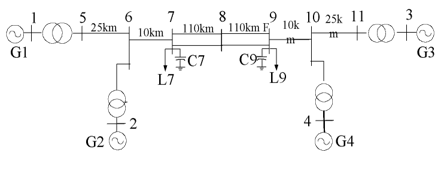
\includegraphics[width=1.4\columnwidth, clip=true]{grid1.png}
	\vspace{-10mm}
	\caption{Our proposed 11-bus system.}
	\label{fig:grid1}
	\vspace{-3mm}
\end{figure*}

We design and implement a 11-bus system including one slack bus (bus $3$), three PV buses (bus $1$, bus $2$, bus $4$) and seven PQ buses (bus $5-11$), as shown in figure \ref{fig:grid1}. All the information of buses, lines and transformers are given in table \ref{tab:bus1}. \ref{tab:line1} and \ref{tab:trans1}.

\begin{table}[]
	\begin{center}
		\begin{tabular}{|l|l|l|l|l|l|}
			\hline
			Bus & Type  & P     & Q    & |v|  & $\theta(degree)$ \\ \hline
			1   & PV    & 7.00  &      & 1.03 &     \\ \hline
			2   & PV    & 7.00  &      & 1.01 &     \\ \hline
			3   & Slack &       &      & 1.03 & 0.0 \\ \hline
			4   & PV    & 7.00  &      & 1.01 &     \\ \hline
			5   & PQ    & 0.00  & 0.00 &      &     \\ \hline
			6   & PQ    & 0.00  & 0.00 &      &     \\ \hline
			7   & PQ    & 9.67  & 1.00 &      &     \\ \hline
			8   & PQ    & 0.00  & 0.00 &      &     \\ \hline
			9   & PQ    & 17.67 & 1.00 &      &     \\ \hline
			10  & PQ    & 0.00  & 0.00 &      &     \\ \hline
			11  & PQ    & 0.00  & 0.00 &      &     \\ \hline
		\end{tabular}
	\end{center}
	\caption{Information of all the buses.}
	\vspace{-3mm}
	\label{tab:bus1}
\end{table}

\begin{table}[]
	\begin{center}
		\begin{tabular}{|l|l|l|l|l|}
			\hline
			Line & Distance(km) & $r_0(pu/km)$ & $x_0(pu/km)$ & $b_0(pu/km)$ \\ \hline
			$L_{56}$ & 25 & 0.0001 & 0.001 & 0.00175 \\ \hline
			$L_{67}$ & 10 & 0.0001 & 0.001 & 0.00175 \\ \hline
			$L_{78}$ & 110 & 0.0001 & 0.001 & 0.00175 \\ \hline
			$L_{89}$ & 110 & 0.0001 & 0.001 & 0.00175 \\ \hline
			$L_{9-10}$ & 10 & 0.0001 & 0.001 & 0.00175 \\ \hline
			$L_{10-11}$ & 25 & 0.0001 & 0.001 & 0.00175 \\ \hline
		\end{tabular}
	\end{center}
	\caption{Information of all the lines.}
	\vspace{-7mm}
	\label{tab:line1}
\end{table}

\begin{table}[H]
	\begin{center}
		\begin{tabular}{|l|l|l|l|}
			\hline
			Transformer & Rated Power(MVA) & Voltage ratio & $z_T$ \\ \hline
			$T_{1}$ & 900 & 1 & j0.15 \\ \hline
			$T_{2}$ & 900 & 1 & j0.15 \\ \hline
			$T_{3}$ & 900 & 1 & j0.15 \\ \hline
			$T_{4}$ & 900 & 1 & j0.15 \\ \hline
		\end{tabular}
	\end{center}
	\caption{Information of all the transformers.}
	\vspace{-4mm}
	\label{tab:trans1}
\end{table}

\subsection{Use GS Method to Find a Initial Solution}
We first calculate the admittance matrix $Y$ using the $r_0$, $x_0$ and $b_0$ value given in table~\ref{tab:line1}, which will then be used to calculate the GS iteration \cite{b3}. In our program, we set the number of iteration to be 100. The algorithm of GS method is shown as following:

\begin{equation}\label{equ:gs}
	V_{i}^{(k+1)}=\frac{1}{y_{ii}}[\frac{P_i-jQ_i}{(V_i^{(k)})^*}-\sum_{n=1}^{i-1}y_{in}V_n^{(k+1)}-\sum_{n=k+1}^Ny_{in}V_n^{(k)}]
\end{equation}

where $k$ represents the number of iteration while $i$ and $n$ represent the column and row in the matrix $Y$ as well as the bus number. We find this is not enough to calculate all the buses. For PV bus, we need to guess an initial value for the voltage phase angle. Then we use the product of our guessed voltage and $Y$ admittance matrix to calculate the guessed power. We take the imaginary part of the power as $Q$ (reactive power) of the PV bus. Then we put it into GS iterations like what PQ bus does above. The difference is that the voltage absolute value is fixed as given and we calculate the phase angle in each iteration as updates. Also, we need to calculate $Q$ for PV bus in each iteration as updates.

\subsection{Use the Solution for NR Method}
After we finish the GS iteration, we have an initial guess of node voltages, which we will use for the calculation of NR method to calculate node powers \cite{b4}. From what we have learned in the class, we first divide $Y$ admittance matrix to $G$ and $B$ matrices, where $G$ is the real part and $B$ matrix is the imaginary part. From equations~\ref{equ:nr1} and~\ref{equ:nr2} we formulate our $f(x)$, which will be used in NR iterations when the $max{f(x)}<\epsilon$. Our $\epsilon$ value here is $10^{-10}$.

\begin{equation}\label{equ:nr1}
	P_{i}=\sum_{n=1}^{N}|V_n||V_i|(G_{in}cos\delta_{in}+B_{in}sin\delta_{in})=P_{Gi}-P_{Di}
\end{equation}

\begin{equation}\label{equ:nr2}
	Q_{i}=\sum_{n=1}^{N}|V_n||V_i|(G_{in}sin\delta_{in}-B_{in}cos\delta_{in})=Q_{Gi}-Q_{Di}
\end{equation}

\begin{equation}
	f(x)=
	\begin{bmatrix}
		P_i-P_{Gi}+P_{Di} \\
		\vdots \\
		P_n-P_{Gn}+P_{Dn} \\
		Q_i-Q_{Gi}+Q_{Di} \\
		\vdots \\
		Q_n-Q_{Gn}+Q_{Dn}
	\end{bmatrix}
    x=
    \begin{bmatrix}
    	\partial_i \\
    	\vdots \\
    	\partial_n \\
    	|V_i| \\
    	\vdots \\
    	|V_n|
    \end{bmatrix}
\end{equation}

$\partial_i$ represents the phase angle for bus $i$, and $|Vi|$ is the absolute value for it. One thing we need to notice is that $i$ to $n$ is from the first bus to the last bus except the slack bus. After we get our GS result, we take the voltage results as our initial guess $x^{(0)}$ for further iteration. Then we need to use the given bus information to calculate the $f(x)$ matrix. The most important part of NR method is to calculate the first order derivation matrix from the $f(x)$. This matrix is named Jacobian matrix, which we do not explain much about here. At last, we need to run our NR iteration through the equation below:

\begin{equation}
	X^{(k+1)}=X^{(k)}-J(x^{(k)})^{-1}\cdot f(x^{(k)})
\end{equation}

We repeat this equation as our NR iterations until we get $max{f(x)}<\epsilon$ as an ending signal. Hence, we get our NR method results.

\subsection{Contingency Analysis}

\begin{figure*}[tp]
	\centering
	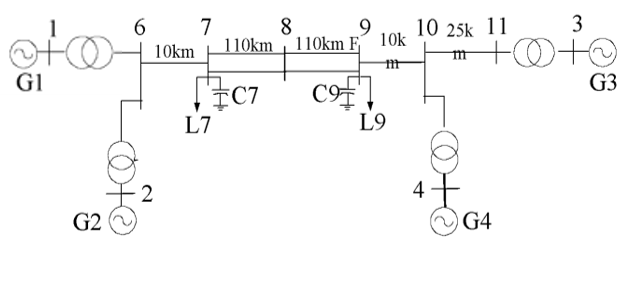
\includegraphics[width=1.25\columnwidth, clip=true]{grid2.png}
	\vspace{-10mm}
	\caption{New grid for contingency analysis.}
	\label{fig:grid2}
	\vspace{-1.5mm}
\end{figure*}

For the contingency analysis, we choose to delete bus $5$ and assume $line_{56}$ disappears. $T_1$ is now connected to bus $6$, as shown in figure~\ref{fig:grid2}. All the other information of the grid remains the same. Now there are $10$ buses in this system including a slack bus, three PV buses and six PQ buses. We then reproduce the same analysis of this new system.

\section{Detailed Solution}
In this section, we provide detailed data of our experiment on both systems. The results of matrix $Y$, GS iteration and NR calculation are given for the original system including node voltages, line currents and power flows. For the new grid without bus $5$, we provide the result of NR calculation and comparison between two systems.

\begin{table*}[]
	\begin{center}
		\setlength{\tabcolsep}{0.4mm}{
			\begin{tabular}{|l|l|l|l|l|l|l|l|l|l|l|}
				\hline
				3.9604-j99.582 & -3.9604+j39.604 &  &  &  &  &  & 0+j60 &  &  &  \\ \hline
				-3.9604+j39.604 & 13.861-j198.58 & -9.901+j99.01 &  &  &  &  &  & 0+j60 &  &  \\ \hline
				& -9.901+j99.01 & 11.701-j114.71 & -1.8002+j18.002 &  &  &  &  &  &  &  \\ \hline
				&  &  & -1.8002+j18.002 & 11.701-j113.21 & -9.901+j99.01 &  &  &  &  &  \\ \hline
				&  &  &  & -9.901+j99.01 & 13.861-j198.58 & -3.9604+j39.604 &  &  & 0+j60 &  \\ \hline
				&  &  &  &  & -3.9604+j39.604 & 3.9604-j99.582 &  &  &  & 0+j60 \\ \hline
				0+j60 &  &  &  &  &  &  & 0-j60 &  &  &  \\ \hline
				& 0+j60 &  &  &  &  &  &  & 0-j60 &  &  \\ \hline
				&  &  &  &  & 0+j60 &  &  &  & 0-j60 &  \\ \hline
				&  &  &  &  &  & 0+j60 &  &  &  & 0-j60 \\ \hline
		\end{tabular}}
	\end{center}
	\caption{The admittance matrix $Y$ for the original system.}
	\vspace{-5.5mm}
	\label{tab:y}
\end{table*}

\subsection{Power Flow Analysis}\label{AA}
We first calculate the admittance matrix $Y$ based on the $r_0$, $x_0$ and $b_0$ value given in table~\ref{tab:line1}. The result of $Y$ is given in table~\ref{tab:y}.

We then calculate the GS iteration based on matrix $Y$. We set the initial voltages for all PQ buses as $1+j0$ and the voltage values of PV buses and slack bus are shown in table~\ref{tab:bus1}. The results of the GS method are shown in table~\ref{tab:gs}.

\begin{table}[H]
	\begin{center}
		\begin{tabular}{|l|l|l|l|}
			\hline
			Bus & |Voltage| & Angle(degree) & Complex \\ \hline
			1 & 1.0300 & -1.5690 & 1.0300-j0.0019 \\ \hline
			2 & 1.0100 & -1.5689 & 1.0100-j0.0019 \\ \hline
			3 & 1.0300 & 0 & 1.0300+j0.0000 \\ \hline
			4 & 1.0100 & -1.5689 & 1.0100-j0.0019 \\ \hline
			5 & 1.0004 & -1.6244 & 0.9989-j0.0536 \\ \hline
			6 & 0.9487 & -1.7116 & 0.9393-j0.1331 \\ \hline
			7 & 0.8885 & -1.8477 & 0.8547-j0.2429 \\ \hline
			8 & 0.5714 & -2.0561 & 0.5054-j0.2665 \\ \hline
			9 & 0.2275 & 3.0700 & 0.2270+j0.0163 \\ \hline
			10 & 0.3340 & -1.6011 & 0.3338-j0.0101 \\ \hline
			11 & 0.6433 & -0.2481 & 0.6236-j0.1580 \\ \hline
		\end{tabular}
	\end{center}
	\caption{Results of GS iteration of the original system.}
	\vspace{-8mm}
	\label{tab:gs}
\end{table}

After that, we use results of GS iteration as a initial guess to calculate NR. In this step, we calculate voltage and power of each node and current and power flow of each line including line losses. The results of node voltage and power are shown in table~\ref{tab:nr1}. Combined with matrix $Y$, we calculate line currents and power flows, as shown in table~\ref{tab:c1} and table~\ref{tab:s1}.

\begin{table}[H]
	\begin{center}
		\begin{tabular}{|l|l|l|l|}
			\hline
			Bus & |Voltage| & Angle(degree) & $P+jQ$ \\ \hline
			1 & 1.03 & 26.922 & 7+j1.810 \\ \hline
			2 & 1.01 & 17.168 & 7+j2.250 \\ \hline
			3 & 1.03 & 0 & 7.187+j1.716 \\ \hline
			4 & 1.01 & -10.171 & 7+j1.918 \\ \hline
			5 & 1.0071 & 20.464 & 0 \\ \hline
			6 & 0.9797 & 10.397 & 0 \\ \hline
			7 & 0.9638 & 2.019 & -9.670-j1 \\ \hline
			8 & 0.9518 & -11.770 & 0 \\ \hline
			9 & 0.9744 & -25.285 & -17.670-j1 \\ \hline
			10 & 0.9851 & -16.904 & 0 \\ \hline
			11 & 1.0090 & -6.619 & 0 \\ \hline
		\end{tabular}
	\end{center}
	\caption{Results of NR calculation of the original system.}
	\vspace{-6mm}
	\label{tab:nr1}
\end{table}

\begin{table}[H]
	\begin{center}
		\begin{tabular}{|l|l|l|l|}
			\hline
			Bus I & Bus J & Current($I_{IJ}$) & Current($I_{JI}$) \\ \hline
			1 & 5 & 6.855294+j1.510179 & -6.855294-j1.510179 \\ \hline
			5 & 6 & 6.855294+j1.510179 & -6.866864-j1.468460 \\ \hline
			2 & 6 & 7.279377-j0.082425 & -7.279377+j0.082425 \\ \hline
			6 & 7 & 14.146241+j1.386035 & -14.148085-j1.369174 \\ \hline
			7 & 8 & 2.078187+j0.014903 & -2.062768+j0.167495 \\ \hline
			8 & 9 & 2.062768-j0.167495 & -2.004024+j0.341979 \\ \hline
			9 & 10 & -13.449209+j4.818059 & 13.455357-j4.80210 \\ \hline
			4 & 10 & 6.486440-j3.093086 & -6.486440+j3.093086 \\ \hline
			10 & 11 & -6.968917+j1.709016 & 6.977727-j1.666474 \\ \hline
			3 & 11 & 6.977727-j1.666474 & -6.977727+j1.666474 \\ \hline
			7 & 0 & -0.071299+j2.022827 & 0 \\ \hline
			9 & 0 & 1.498220+j3.171676 & 0 \\ \hline
		\end{tabular}
	\end{center}
	\caption{Results of current in each line.}
	\vspace{-6mm}
	\label{tab:c1}
\end{table}

\begin{table*}[ht]
	\begin{center}
		\begin{tabular}{|l|l|l|l|l|}
			\hline
			Bus I & Bus J & Power($S_{IJ}$) & Power($S_{JI}$) & Line Loss \\ \hline
			1 & 5 & 7.000000+j1.810135 & -7.000000-j0.988874 & 0.000000+j0.821262 \\ \hline
			5 & 6 & 7.000000+j0.988874 & -6.876701+j0.200930 & 0.123299+j1.189803 \\ \hline
			2 & 6 & 7.000000+j2.249742 & -7.000000-j1.366474 & 0.000000+j0.883269 \\ \hline
			6 & 7 & 13.876701+j1.165544 & -13.674644+j0.838505 & 0.202058+j2.004050 \\ \hline
			7 & 8 & 2.002322+j0.056203 & -1.954598+j0.244420 & 0.047724+j0.300623 \\ \hline
			8 & 9 & 1.954598-j0.244420 & -1.907910+j0.532728 & 0.046688+j0.288309 \\ \hline
			9 & 10 & -13.854180+j1.352375 & 14.058299+j0.672013 & 0.204119+j2.024387 \\ \hline
			4 & 10 & 7.000000+j1.918092 & -7.000000-j1.057407 & 0.000000+j0.860685 \\ \hline
			10 & 11 & -7.058299+j0.385394 & 7.187059+j0.858704 & 0.128760+j1.244098 \\ \hline
			3 & 11 & 7.187059+j1.716468 & -7.187059-j0.858704 & 0.000000+j0.857763 \\ \hline
			7 & 0 & 0.000000-j1.950911 & 0 & 0.000000-j1.950911 \\ \hline
			9 & 0 & 0.000000-j3.417832 & 0 & 0.000000-j3.417832 \\ \hline
		\end{tabular}
	\end{center}
	\caption{Results of power flow in each line.}
	\vspace{-4mm}
	\label{tab:s1}
\end{table*}

\subsection{Contingency Analysis}
After analyzing the old grid, we analyze the new grid with same approaches. We only present node voltages and powers, current flows and power flows. The node voltages and powers are shown in table~\ref{tab:nr2} and values of line currents and power flow are shown in table~\ref{tab:c2} and table~\ref{tab:s2}.

\begin{table}[H]
	\vspace{-2mm}
	\begin{center}
		\begin{tabular}{|l|l|l|l|}
			\hline
			Bus & |Voltage| & Angle(degree) & $P+jQ$ \\ \hline
			1 & 1.03 & 37.135541 & 7+j2.419799 \\ \hline
			2 & 1.01 & 37.265257 & 7+j1.176506 \\ \hline
			3 & 1.03 & 0 & 7.073890+j1.498509 \\ \hline
			4 & 1.01 & -9.845945 & 7+j1.457941 \\ \hline
			6 & 0.997298 & 30.614072 & 0 \\ \hline
			7 & 0.973899 & 22.440945 & -9.670-j1 \\ \hline
			8 & 0.932464 & -6.768899 & 0 \\ \hline
			9 & 0.987512 & -20.604789 & -17.670-j1 \\ \hline
			10 & 0.992685 & -16.528177 & 0 \\ \hline
			11 & 1.012245 & -6.492871 & 0 \\ \hline
		\end{tabular}
	\end{center}
	\caption{Results of NR calculation of the new system.}
	\vspace{-6mm}
	\label{tab:nr2}
\end{table}

\begin{table*}[ht]
	\begin{center}
		\begin{tabular}{|l|l|l|l|l|}
			\hline
			Bus I & Bus J & Power($S_{IJ}$) & Power($S_{JI}$) & Line Loss \\ \hline
			1 & 6 & 7.000000+j2.41979 & -7.000000-j1.558024 & 0.000000+j0.861775 \\ \hline
			2 & 6 & 7.000000+j1.176506 & -7.000000-j0.353316 & 0.000000+j0.823190 \\ \hline
			6 & 7 & 14.000000+j1.911340 & -13.799230+j0.079359 & 0.200770+j1.990699 \\ \hline
			7 & 8 & 4.129230+j0.912449 & -3.919802+j1.006853 & 0.209428+j1.919302 \\ \hline
			8 & 9 & 1.959901-j0.503427 & -1.909076+j0.834122 & 0.050824+j0.330695 \\ \hline
			9 & 10 & -6.925924+j0.421201 & 6.975302+j0.055431 & 0.049379+j0.476632 \\ \hline
			4 & 10 & 7.000000+j1.457941 & -7.000000-j0.622638 & 0.000000+j0.835304 \\ \hline
			10 & 11 & -6.950605+j0.511775 & 7.073890+j0.677109 & 0.123285+j1.188884 \\ \hline
			3 & 11 & 7.073890+j1.498509 & -7.073890-j0.677109 & 0.000000+j0.821401 \\ \hline
			7 & 0 & 0.000000-j1.991808 & 0 & 0.000000-j1.991808 \\ \hline
			9 & 0 & 0.000000-j3.510645 & 0 & 0.000000-j3.510645 \\ \hline
		\end{tabular}
	\end{center}
	\caption{Power results of the new grid.}
	\vspace{-8mm}
	\label{tab:s2}
\end{table*}

\begin{table}[H]
	\begin{center}
		\begin{tabular}{|l|l|l|l|}
			\hline
			Bus I & Bus J & Current($I_{IJ}$) & Current($I_{JI}$) \\ \hline
			1 & 6 & 6.836220+j2.229933 & -6.836220-j2.229933 \\ \hline
			2 & 6 & 6.221057+j3.269534 & -6.221057-j3.269534 \\ \hline
			6 & 7 & 13.057276+j5.499468 & -13.064973-j5.484081 \\ \hline
			7 & 8 & 4.276466+j0.752545 & -4.301671-j0.576781 \\ \hline
			8 & 9 & 2.150835+j0.288391 & -2.106808-j0.110299 \\ \hline
			9 & 10 & -6.714961+j2.068952 & 6.720473-j2.052537 \\ \hline
			4 & 10 & 6.581772-j2.607391 & -6.581772+j2.607391 \\ \hline
			10 & 11 & -6.859173+j1.497682 & 6.867854-j1.454864 \\ \hline
			3 & 11 & 6.867854-j1.454864 & -6.867854+j1.454864 \\ \hline
			7 & 0 & -0.780712+j1.890314 & 0 \\ \hline
			9 & 0 & 1.251090+j3.327626 & 0 \\ \hline
		\end{tabular}
	\end{center}
	\caption{Current results of the new grid.}
	\vspace{-6mm}
	\label{tab:c2}
\end{table}

\subsection{Comparison}
Compared to the original grid, there are some changes in the new grid. For each PQ bus ($6-11$), the absolute value of voltage slightly increases while the phase value changes a lot. For the slack bus and all the PV buses ($1-4$), the phase value of voltage and input power changes a little bit. For the power flow changes in each line, if the line is closer to the deleted bus, the changes in the power flow, line losses and line current will be greater. In summary, the failure of bus $5$ does not cause significant changes in the new system.


\section{Conclusions}
In this project, we design and implement a 11-bus power system and finish power flow analysis of the proposed grid. We utilize GS method to find a initial solution, which is then used for the NR method to calculate the final results including node voltages, line currents and power losses. We also choose bus $5$ for contingency analysis. Assuming this bus is failing and the corresponding line disappears, we finish the same process of analysis of the new system. The result shows that the failure of bus $5$ does not cause significant changes in most nodes and lines and our system has strong ability to deal with bus failure.

%\section*{Acknowledgment}
%
%The preferred spelling of the word ``acknowledgment'' in America is without 
%an ``e'' after the ``g''. Avoid the stilted expression ``one of us (R. B. 
%G.) thanks $\ldots$''. Instead, try ``R. B. G. thanks$\ldots$''. Put sponsor 
%acknowledgments in the unnumbered footnote on the first page.

\newpage
\begin{thebibliography}{00}
\bibitem{b1} Albadi M, Volkov K. Power flow analysis[J]. Computational Models in Engineering, 2020.
\bibitem{b2} Sorooshian K. Load flow and contingency analysis in power systems[J]. 1984.
\bibitem{b3} Wikipedia. Gauss–Seidel method. [Online.] Available: https://en.wikipedia.org/wiki/Gauss-Seidel$\_$method, 2021.
\bibitem{b4} Wikipedia. Newton's method. [Online.] Available: https://en.wikipedia.org/wiki/Newton$\%$27s$\_$method, 2021.
\end{thebibliography}

\appendices
\section{Implementation of the System}
\begin{lstlisting}
function [node_result,s_result] = PowerSystem
                                  % main function
[node] = OpenNode; 
[nn,mn] = size(node);             % load node info

[line] = OpenLine;
[nl,ml] = size(line);              % load line info

[node,line,nPQ,nPV,nodenum,PH,PV,PQ] = Num(node,line);
                                 % rearrange nodes
Y = sparse(Yij(node,line))          % calculate Y

[U] = Gauss_Seidel(Y,node,nPQ,nPV)
[U1] = abs(U)              % return the results of GS
[U2] = angle(U)

[node_result,s_result] =Newton_Raphson(U1,Y,node,nPQ,nPV,line,nodenum);
                                   % calculate NR
Result_Write(node_result,s_result,node,line);
                           % write results in a txt file
\end{lstlisting}

\section{Admittance Matrix}
\begin{lstlisting}
function Y = Yij(node,line)

[nn,mn]=size(node);
[nl,ml]=size(line);

Y=zeros(nn,nn);            % set initial value to be 0 

for k=1:nl    
    I=line(k,1);   
    J=line(k,2);    
    Zt=line(k,3)+j*line(k,4);      % load line info 
    if Zt~=0
        Yt=1/Zt;          % no Yt for grounded lines
    end
    Ym=line(k,5)+j*line(k,6);     % calculate G+B
    K=line(k,7);                % load voltage ratio
    
    if (K==0)&(J~=0)
        Y(I,I)=Y(I,I)+Yt+Ym;
        Y(J,J)=Y(J,J)+Yt+Ym;           
        Y(I,J)=Y(I,J)-Yt;
        Y(J,I)=Y(I,J);    
    end

    if (K==0)&(J==0)              % grounded line
        Y(I,I)=Y(I,I)+Ym;
    end        

    if K>0                        % trans line: to i       
        Y(I,I)=Y(I,I)+Yt+Ym;        
        Y(J,J)=Y(J,J)+Yt/K/K;        
        Y(I,J)=Y(I,J)-Yt/K;        
        Y(J,I)=Y(I,J);    
    end        
    
    if K<0                        % trans line: to j
        Y(I,I)=Y(I,I)+Yt+Ym;        
        Y(J,J)=Y(J,J)+K*K*Yt;        
        Y(I,J)=Y(I,J)+K*Yt;        
        Y(J,I)=Y(I,J);    
    end  
end
\end{lstlisting}

\section{GS Method}
\begin{lstlisting}
function [U] = Gauss_Seidel(Y,node,nPQ,nPV)

[nn,mn]=size(node);
U=zeros(nn,1);             % initialize voltage matrix
Umax1=zeros(nn,1);            % Umax for max error
Umax2=zeros(nn,1);
k=100;                            % 100 iterations

for i=1:nn
U(i,1) = 1;                   % initial value to be 1
end

while k
    for i=1:nn
        switch node(i,6)             % node type
            case 1                    % 1 for PQ
                [U1] = PQ(i,U,node,Y,nPQ);
                U(i,1)=U1(i,1);
            case 2                    % 2 for PV
                [U2] = PV(i,U,node,Y,nPV);
                U(i,1)=U2(i,1); 
            case 3                   % 3 for slack
                U(i,1)=node(i,2)*cos(node(i,3))-node(i,2)*sin(node(i,3))*sqrt(-1);
        end  
    end
    k=k-1;
end
\end{lstlisting}

\section{NR Method}
\begin{lstlisting}
function [node_result,s_result] =Newton_Raphson(U,Y,node,nPQ,nPV,line,nodenum)
[nn,mn] = size(node);

EPS = 1.0e-10;                  % precision of error

for t = 1:1000                 % 1000 iteration max

    [dP,dQ] = DPQ(Y,node,nPQ,nPV);                    
                         % calculate error of P and Q
    Jac = sparse(Jac_NR(node,Y,nPQ));
                             % calculate Jac matrix
    UD = zeros(nPQ,nPQ); 
    for i = 1:nPQ
        UD(i,i) = U(i,1);  % voltage diagonal matrix
    end

    dAngU = Jac \ [dP;dQ];
    dAng = dAngU(1:nn-1,1);     % phase correction
    dU = UD*(dAngU(nn:nn+nPQ-1,1));
                               % voltage correction
    node(1:nPQ,2) = node(1:nPQ,2) - dU;
                                     % fix voltage
    node(1:nn-1,3) = node(1:nn-1,3) - dAng;
                                      % fix phase
    if (max(abs(dU))<EPS)&(max(abs(dAng))<EPS)
        break
    end                          % fulfill precision?
end

node = PQ_NR(node,Y,nPQ,nPV)% P and Q for each node

[node,line] = ReNum(node,line,nodenum);
                            % recover node numbers
YtYm = YtYm_NR(line);      % Yt and Ym for each line

node_result = Node_result(node);    % node values
s_result = S_result(node,line,YtYm); % line values
\end{lstlisting}

\end{document}
